\section{Radioactivity: fundamentals}

%\frame{\tableofcontents[currentsection]}

\begin{frame}{Ionizing radiation}

\alert{Radiation with enough energy to detach electrons from atoms or molecules, thus ionizing them}

\pause
\vskip-2cm
\centering
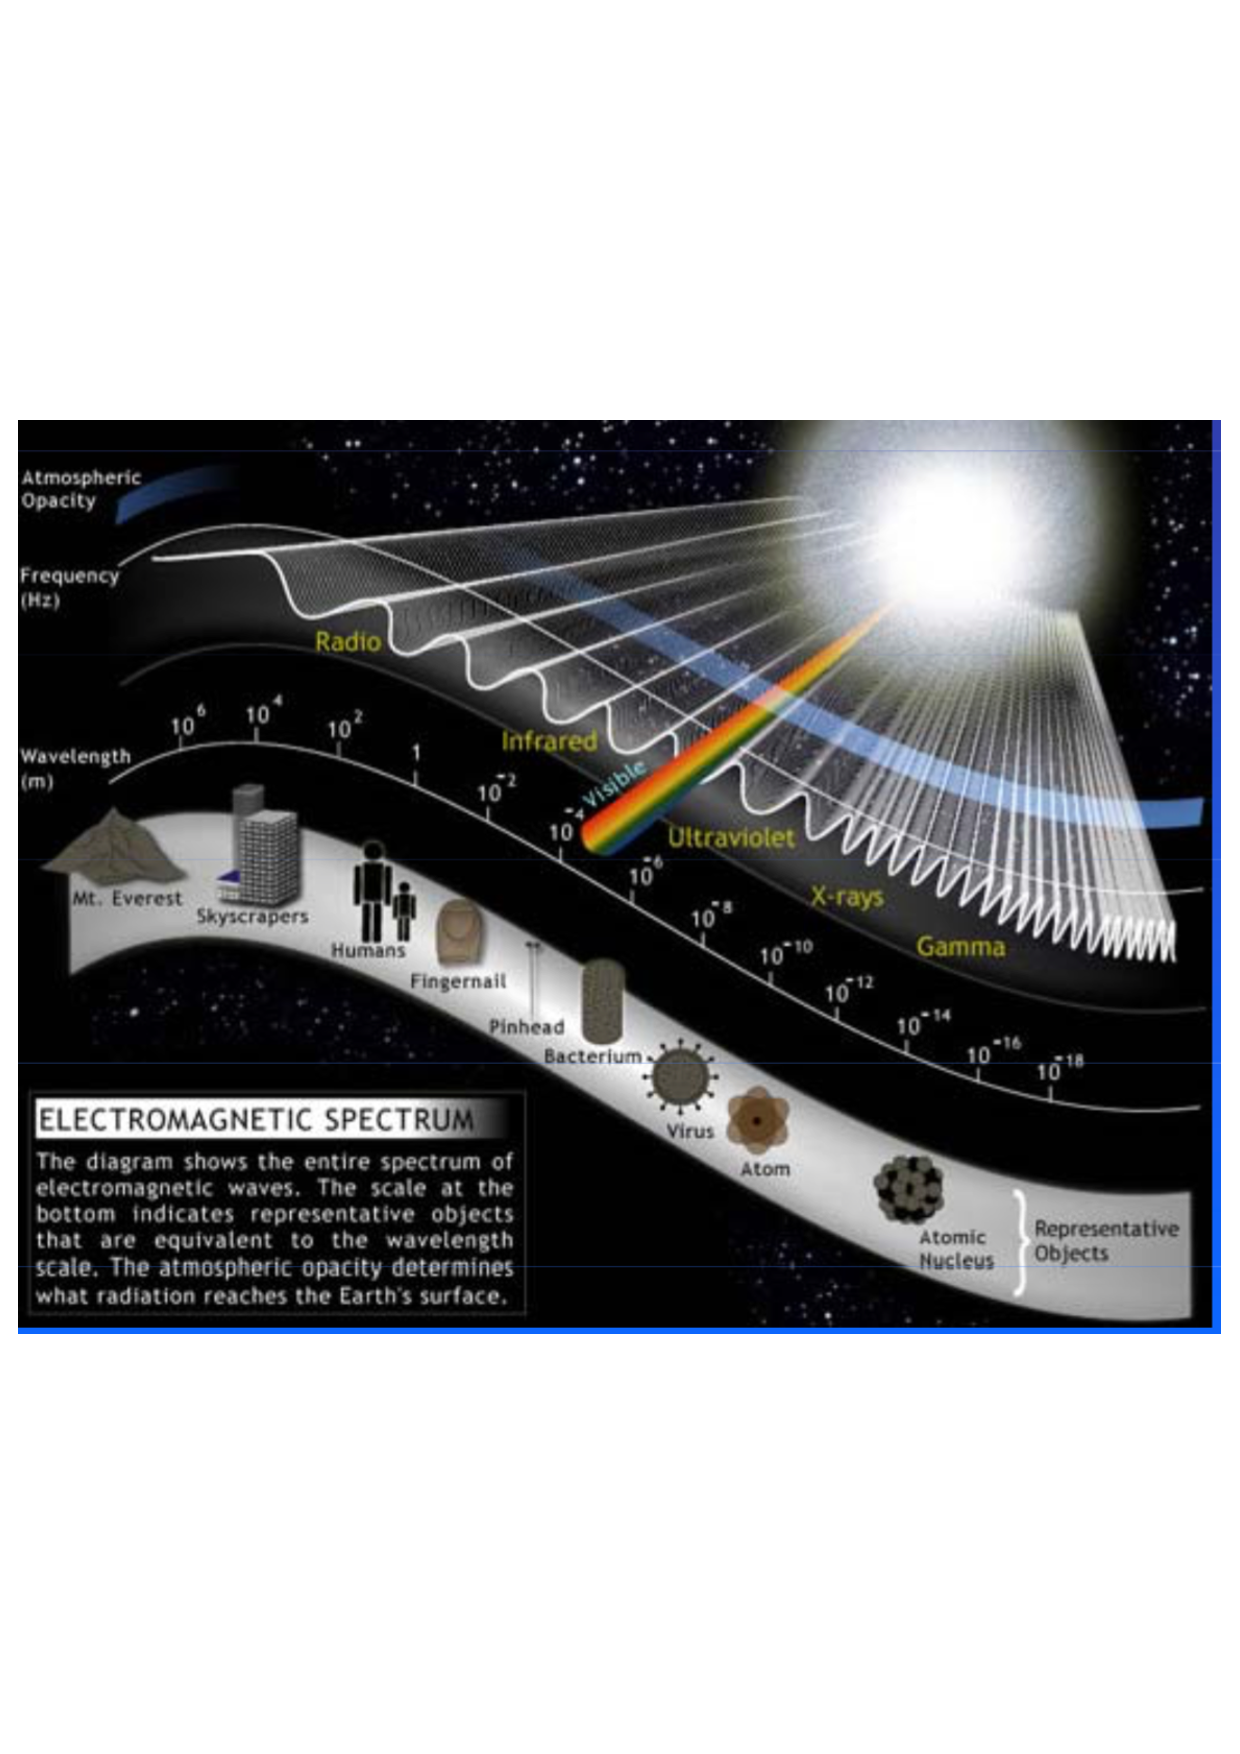
\includegraphics[scale=0.3]{figures/20160218_rsw_emspectrum.pdf}

\vskip-2cm
\begin{itemize}
\item Energies: keV and MeV
\item Decay modes: alpha, beta and gamma
\end{itemize}

\end{frame}

\begin{frame}{Numbers and names}

\begin{table}[H]
%\caption{}
%\label{tab::}
\vskip -0.5cm
\begin{center}
  \begin{tabular}{p{3cm}p{4cm}c}
  \toprule
Symbol      & Definition & Fingerprint   \\ \otoprule 
$Z$ (atomic number) & The atomic number of an atom is the number of protons it contains & ATOM \\
$A$ (mass number; atomic mass number or nucleon number) &  Total number of protons and neutrons (together known as nucleons) in an atomic nucleus & ISOTOPE  \\ \bottomrule
\end{tabular}
\end{center}
\end{table}

\pause \centering \alert{radon: $^{222}_{86}$Rn; $^{220}_{86}$Rn; $^{219}_{86}$Rn}

\end{frame}

\begin{frame}{Decay modes}

\alert{Alpha decay: Emission of an alpha particle ($^{4+}_{2}$He) by a nucleus}

\begin{exampleblock}{Characteristics of the alpha decay mode}

\begin{itemize}
\item High enery (MeV)
\item Heavy particles: they can be stopped in some cm 
\item Elements heavy nucleus
\item Examples: $^{222}_{86}$Rn, $^{238}_{92}$U, $^{210}_{84}$Po
\end{itemize}

\end{exampleblock}

\end{frame}

\begin{frame}{Decay modes}

\alert{Example of alpha spectrum}

\centering
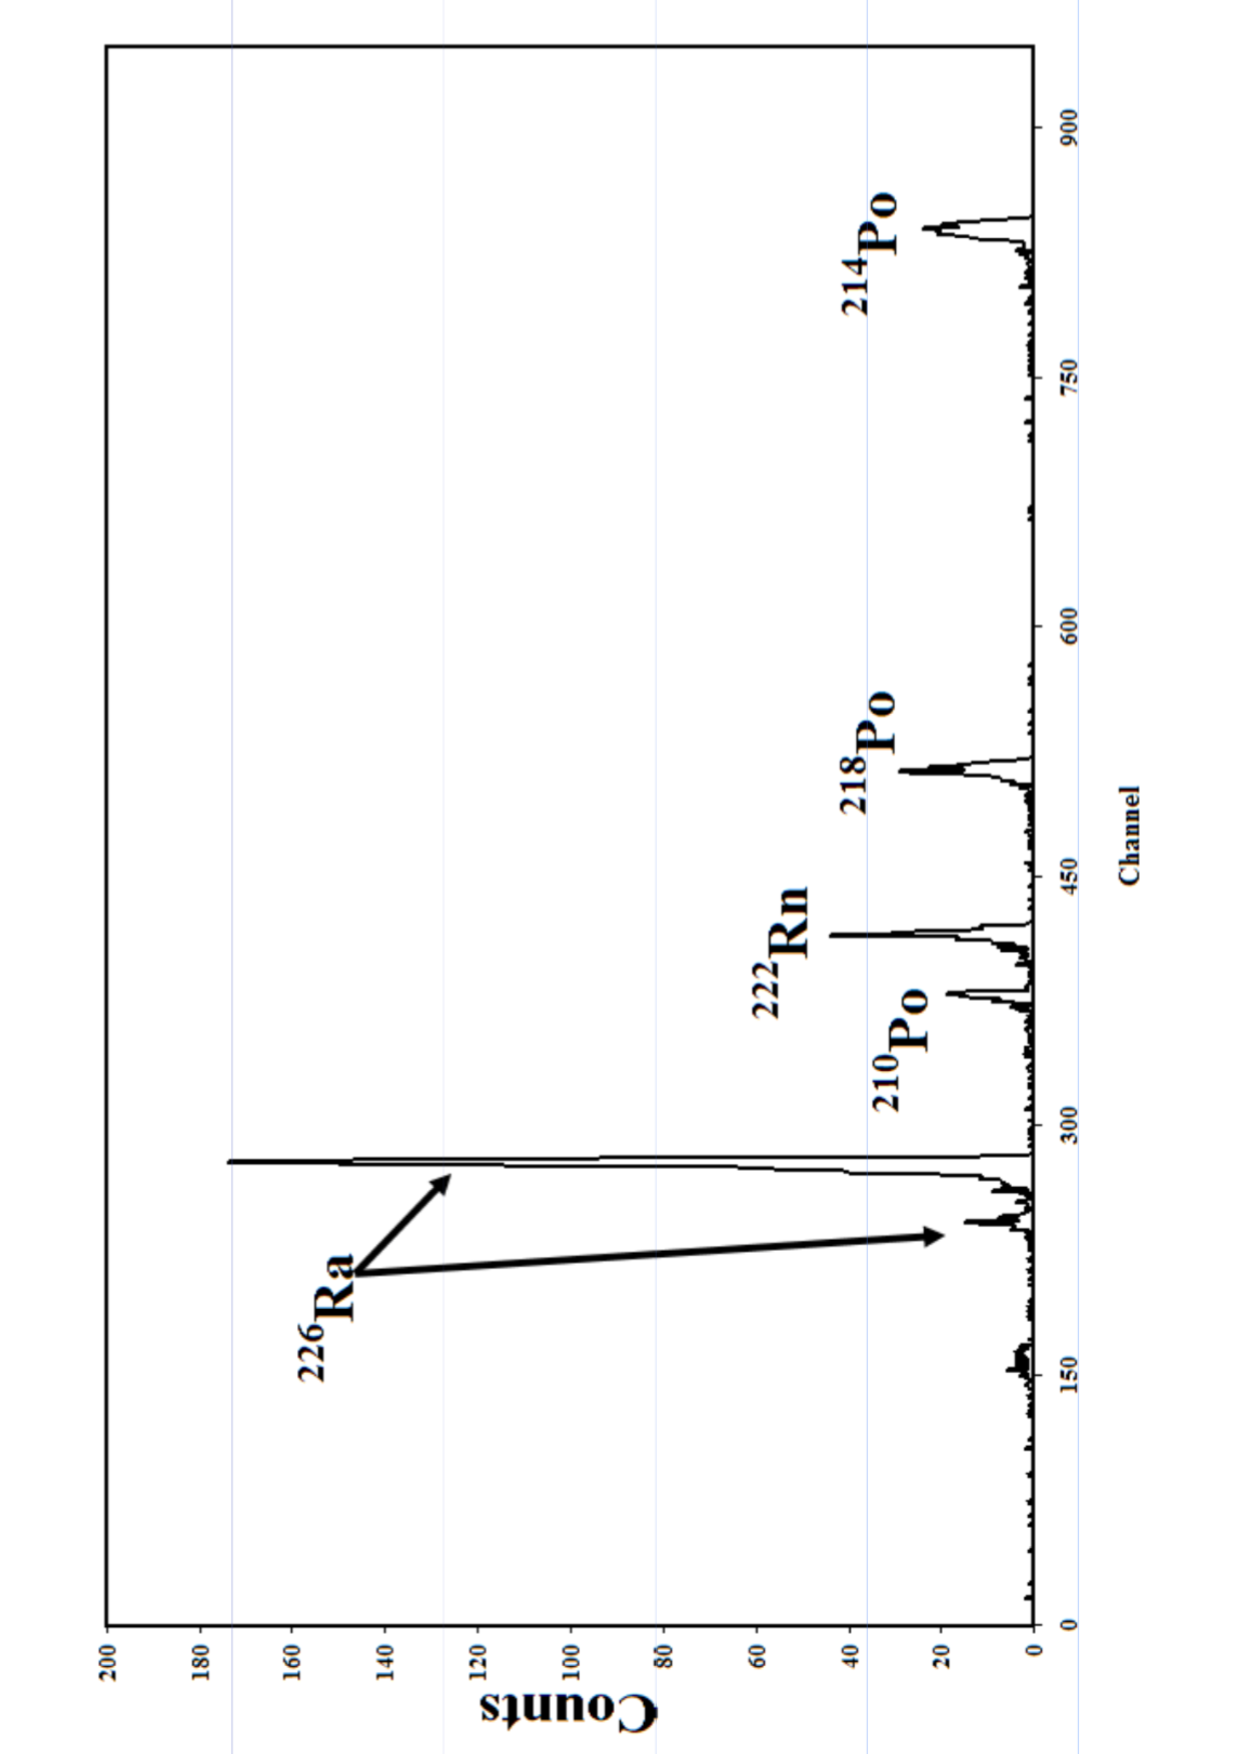
\includegraphics[scale=0.3,angle=-90]{figures/20160218_rsw_alphaspectrum.pdf}

\end{frame}

\begin{frame}{Decay modes}

\alert{Beta decay: Emission of beta particle (positive or negative) by a nucleus. Also electron capture by a nucleus.}

\begin{exampleblock}{Characteristics of the beta decay mode}

\begin{itemize}
\item Less energy than alpha emission 
\item Longer distance before stopping 
\item Continuous spectrum of energy
\item Examples: $^{3}_{1}$H, $^{90}_{38}$Sr
\end{itemize}

\end{exampleblock}

\end{frame}

\begin{frame}{Decay modes}

\alert{Example of beta spectrum}

\vskip-4cm
\centering
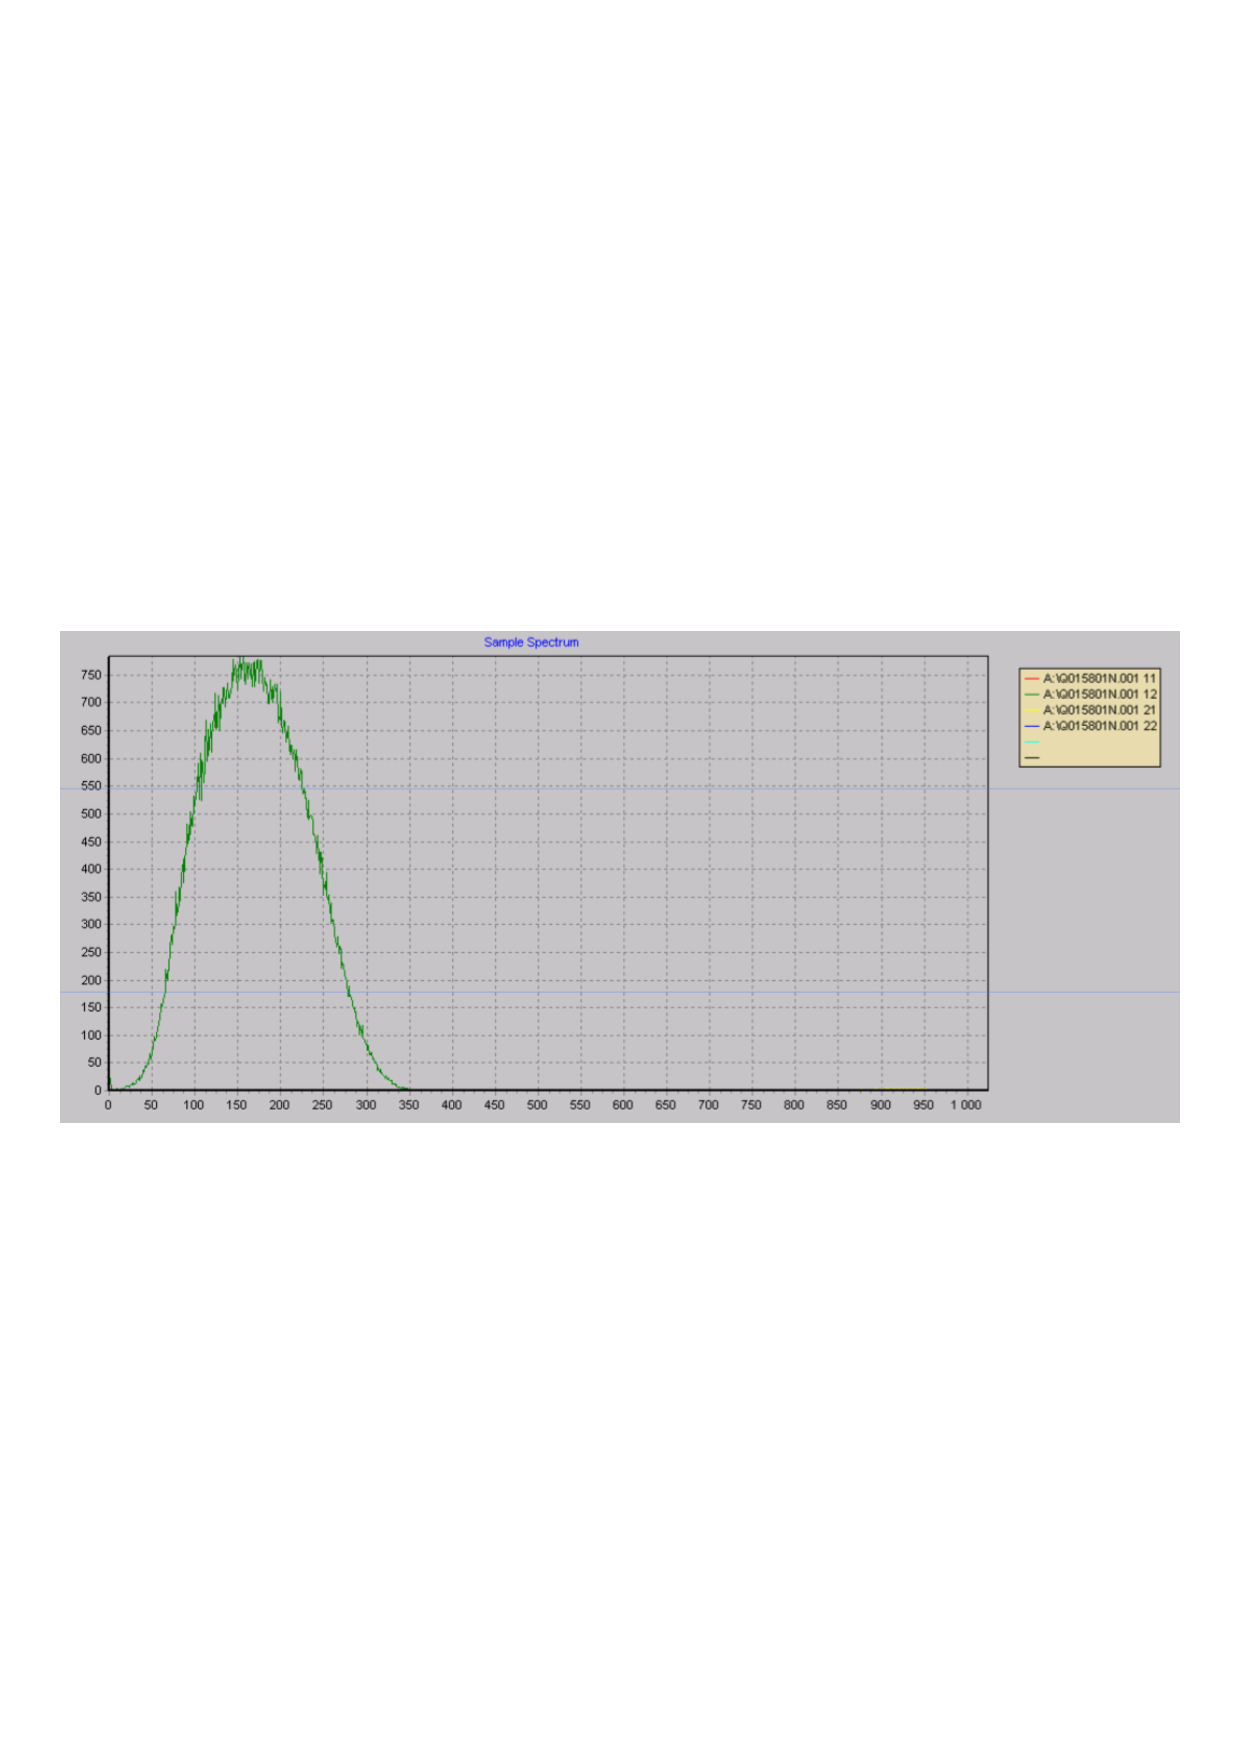
\includegraphics[scale=0.5]{figures/20160218_rsw_betaspectrum.pdf}

\end{frame}

\begin{frame}{Decay modes}

\alert{Gamma decay: Photon’s emission by a nucleus when reaching steady state of energy.}

\begin{exampleblock}{Characteristics of the gamma decay mode}

\begin{itemize}
\item Photons with different energies
\item X Rays 
\item Gamma Rays (with different
energies)
\item Gamma rays = Nucleus 
\item X Rays = Atomic crust
\item Examples: $^{99}_{43}$Tc, $^{60}_{27}$Co
\end{itemize}

\end{exampleblock}

\end{frame}

\begin{frame}{Decay modes}

\alert{Example of gamma spectrum}

%\vskip-2cm
\centering
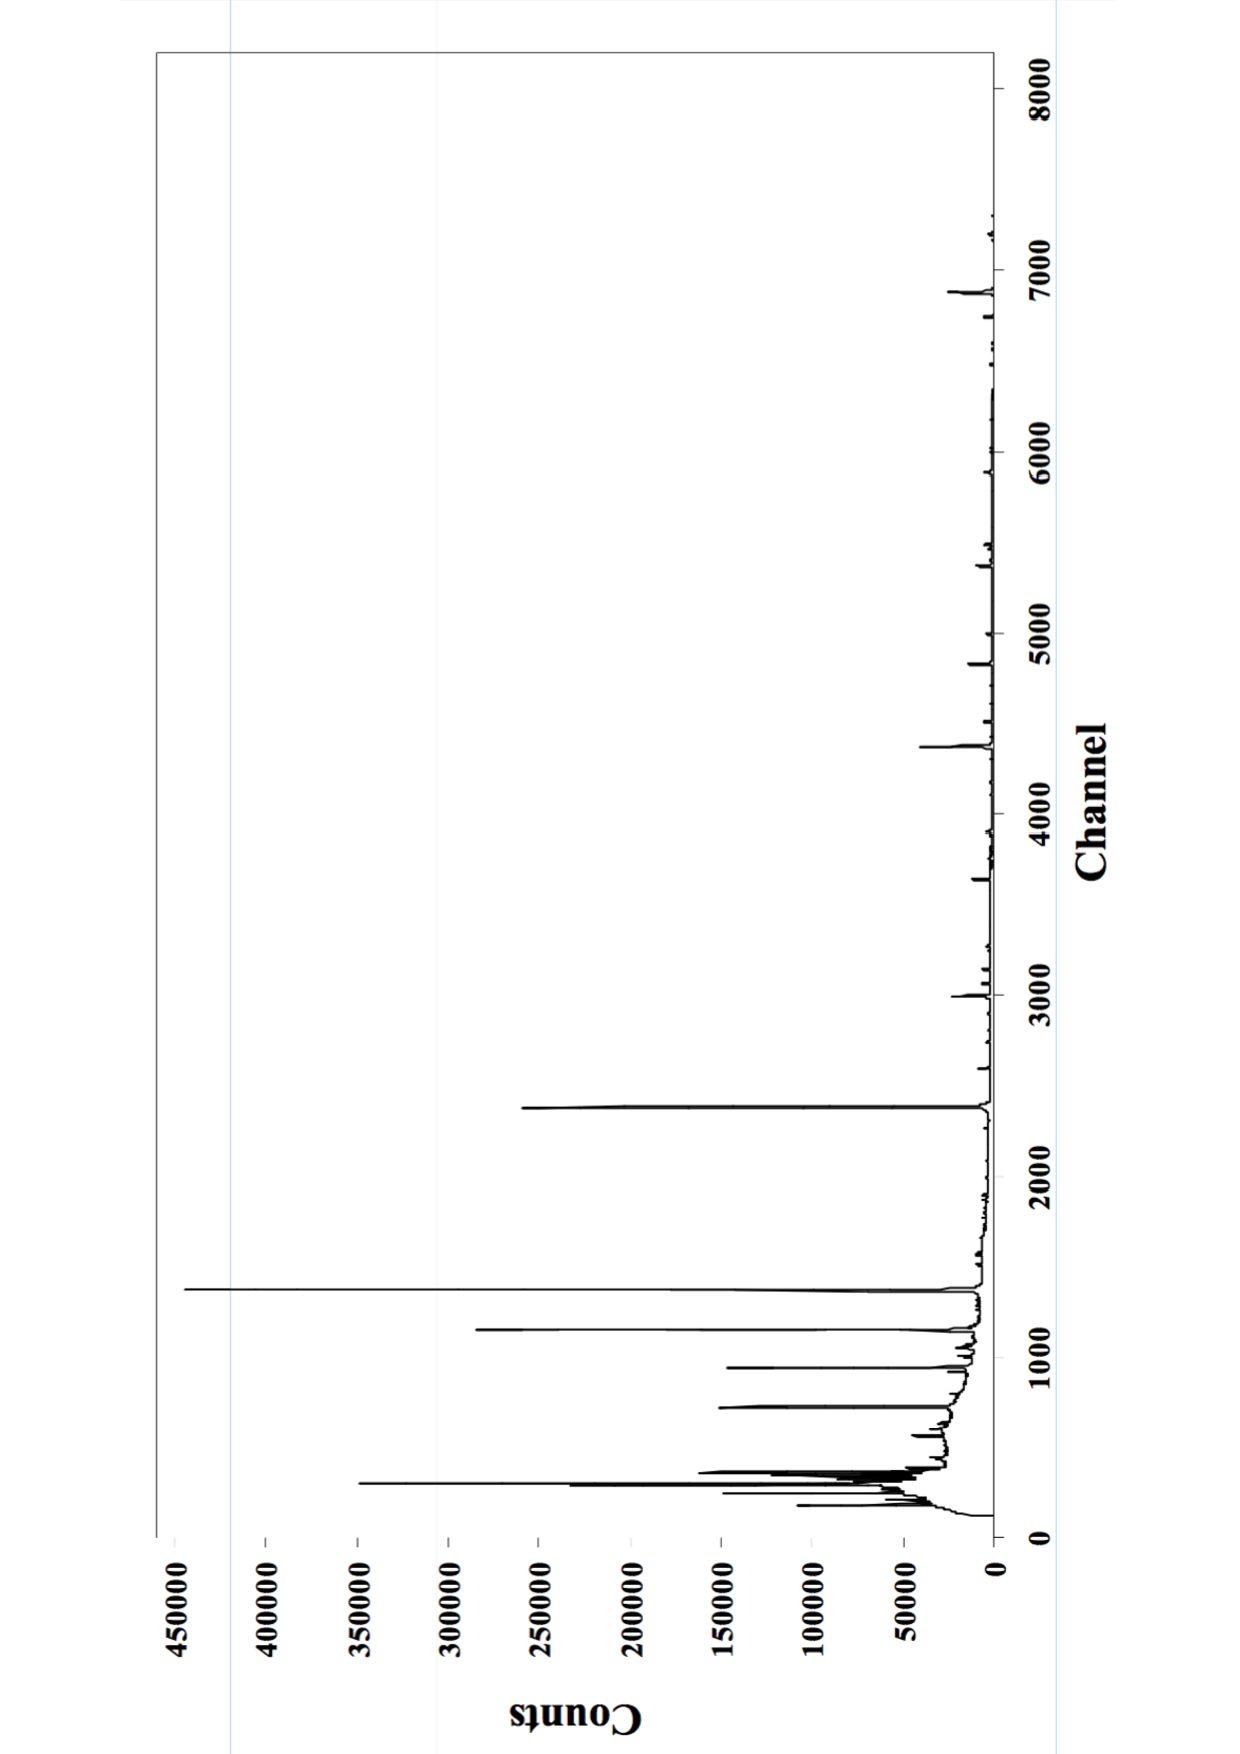
\includegraphics[scale=0.35, angle=-90]{figures/20160218_rsw_gammaspectrum.pdf}

\end{frame}

\begin{frame}{Penetration power}

\centering
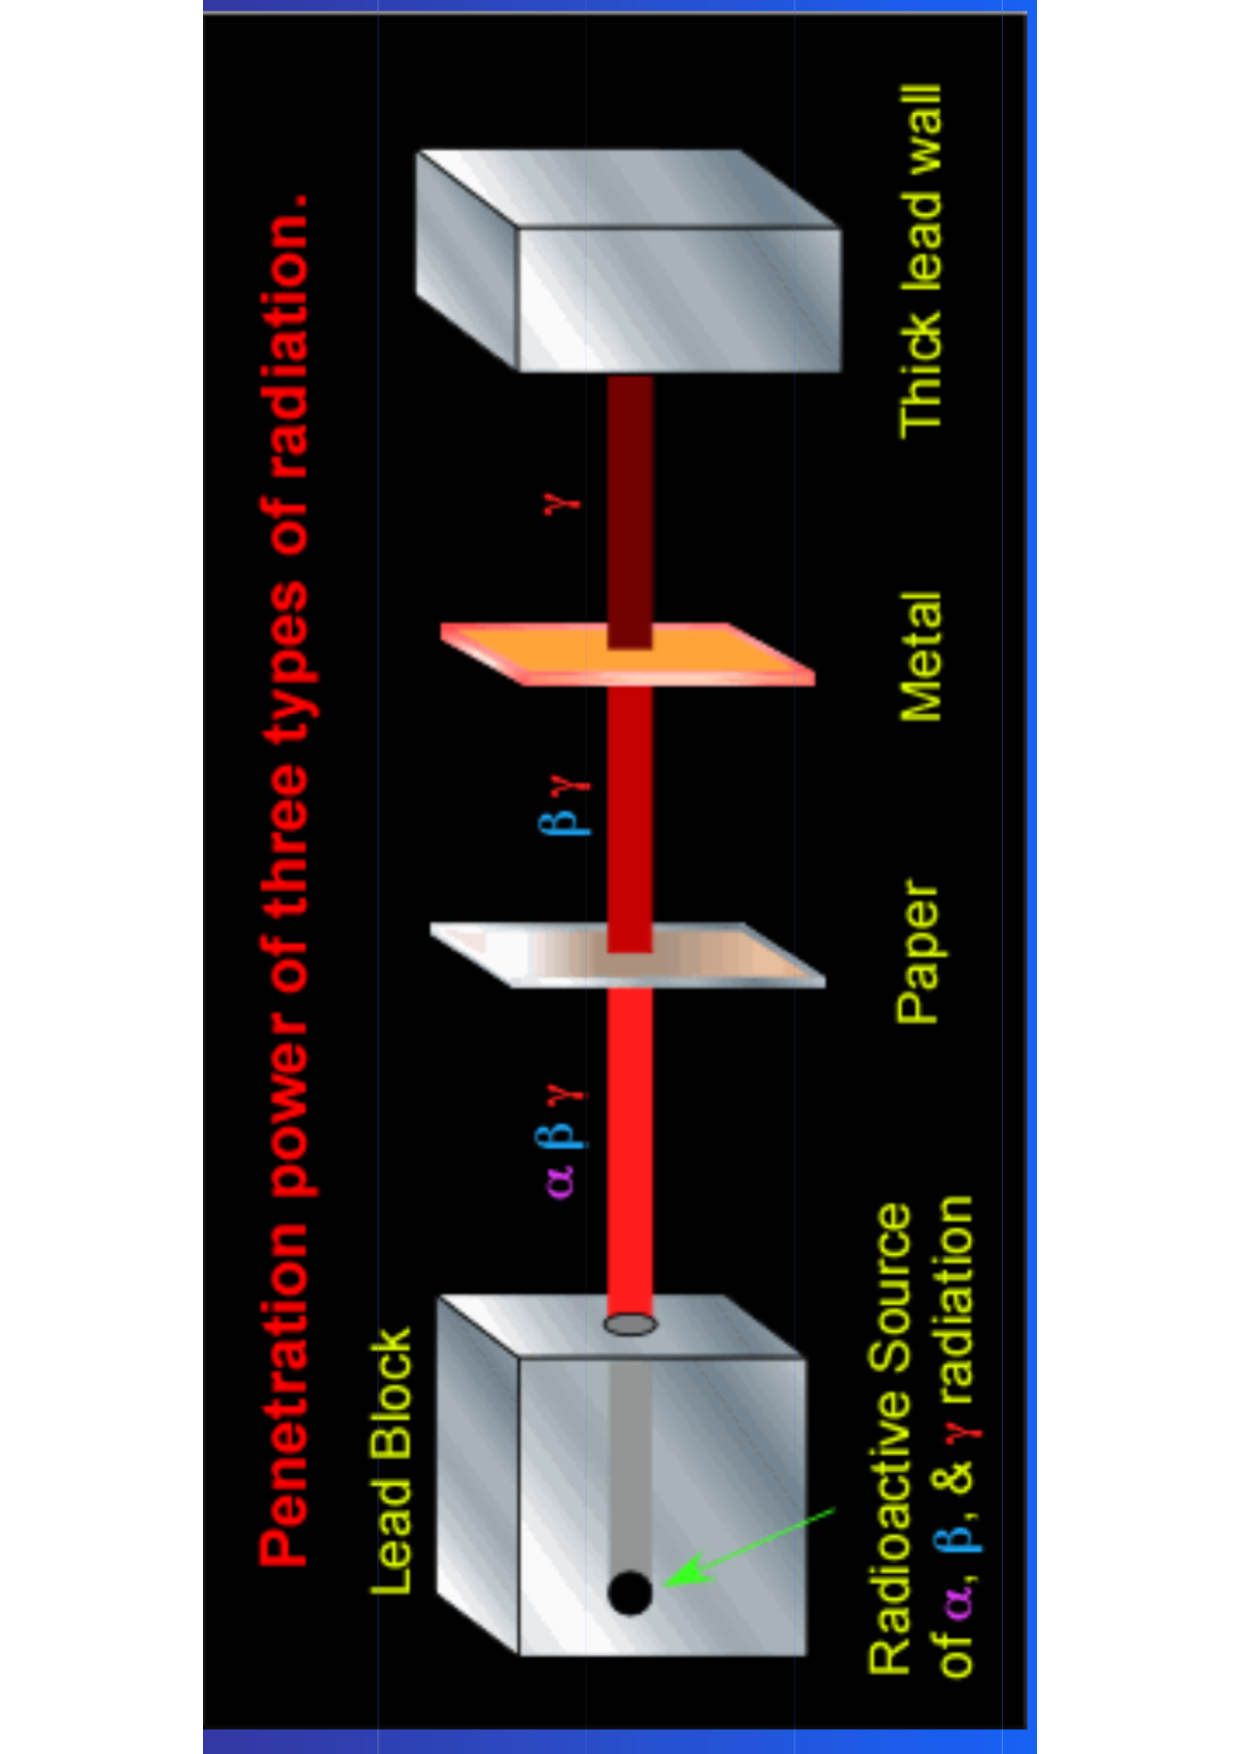
\includegraphics[scale=0.35, angle=-90]{figures/20160218_rsw_penetration.pdf}

\end{frame}

\begin{frame}{Definitions}

\begin{exampleblock}{}

\begin{itemize}
	\item Activity (A): Number of disintegrations per second
\item Half life ($T_{1/2}$): Neccesary time for an isotope to decrease its nucleus by half (s)
\item Decay constant ($\lambda$): Probability of disintegration by time (s$^{-1}$)
\item Decay chain: chained series of transformations (4 Natural decay chains)
\end{itemize}

\end{exampleblock}

\end{frame}

\begin{frame}{Units}

\begin{exampleblock}{}

\begin{itemize}
	\item Becquerel (Bq) : unit of activity in the International System of
Units: 1Bq = 1 DPS (disintegration / second) \item Curie(Ci):Old unit of activity: 1Ci=$3.7\cdot10^{10}$ Bq
\item Concentration : Bq/kg, Bq/l, Bq/m3
\item Sievert (Sv) : Unit for equivalent dose
\item Working Level Month (WLM): Occupational exposure (1 WLM is approximately equivalent to an exposure of 150 Bq m$^{-3}$ in a year)
\end{itemize}

\end{exampleblock}

\end{frame}

\begin{frame}{Exponential's decay law}

\centering \alert{$A=A_0e^{-\lambda\cdot t}$}

\centering
\vskip-1.5cm
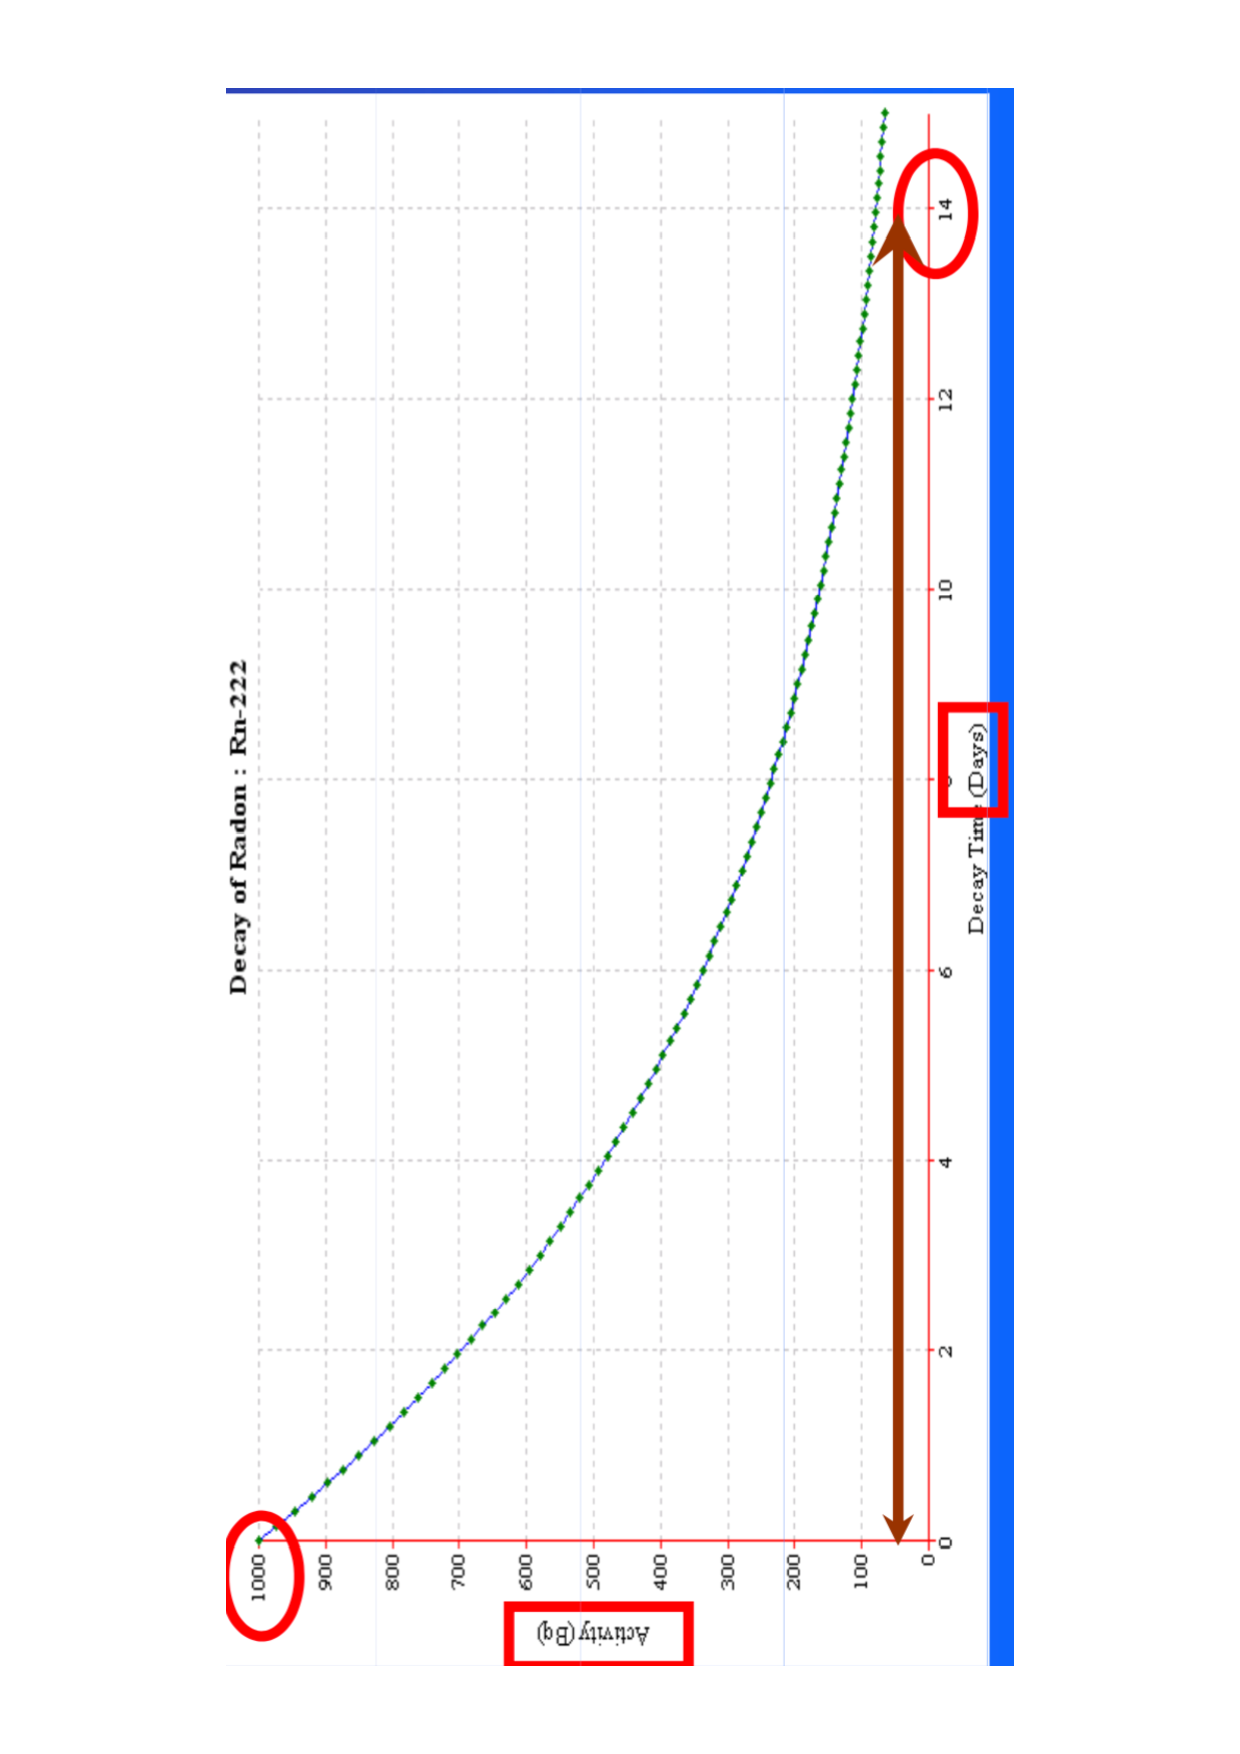
\includegraphics[scale=0.4,angle=-90]{figures/20160218_rsw_exponentiallaw.pdf}

\end{frame}

\begin{frame}{Half-lives}

\begin{table}[H]
%\caption{}
%\label{tab::}
\vskip -0.5cm
\begin{center}
  \begin{tabular}{cc}
  \toprule
Isotope      & Half life     \\ \otoprule 
$^{238}$U   & $4.5\cdot 10^9$ y \\ 
$^{14}$C   & 5730 y \\
$^{3}$H   & 12.4 y \\
$^{131}$I   & 8.03 d \\
$^{222}$Rn   & 3.8 d \\ 
$^{99}$Tc   & 6 h \\ 
$^{219}$Rn   & 3.96 s \\ \bottomrule
\end{tabular}
\end{center}
\end{table}

\end{frame}

\begin{frame}{Natural decay series}

\begin{table}[H]
%\caption{}
%\label{tab::}
\vskip -0.5cm
\begin{center}
  \begin{tabular}{llll}
  \toprule
Series                                     & Start     & Half life (y)  & Final product \\ \otoprule 
Thorium & $^{232}$Th & $1.41\cdot 10^{10}$ & $^{208}$Pb \\
Neptunium & $^{237}$Np & $2.14\cdot 10^{6}$ & $^{209}$Pb \\  
Uranium & $^{238}$U & $4.51\cdot 10^{9}$ & $^{206}$Pb \\
Actinium & $^{235}$U & $7.18\cdot 10^{8}$ & $^{207}$Pb \\ \bottomrule
\end{tabular}
\end{center}
\end{table}

\centering
\alert{{\large Earth's age: $4.65\cdot 10^{9}$}}

\end{frame}

\begin{frame}{Natural decay series Uranium}

\begin{figure}
\centering
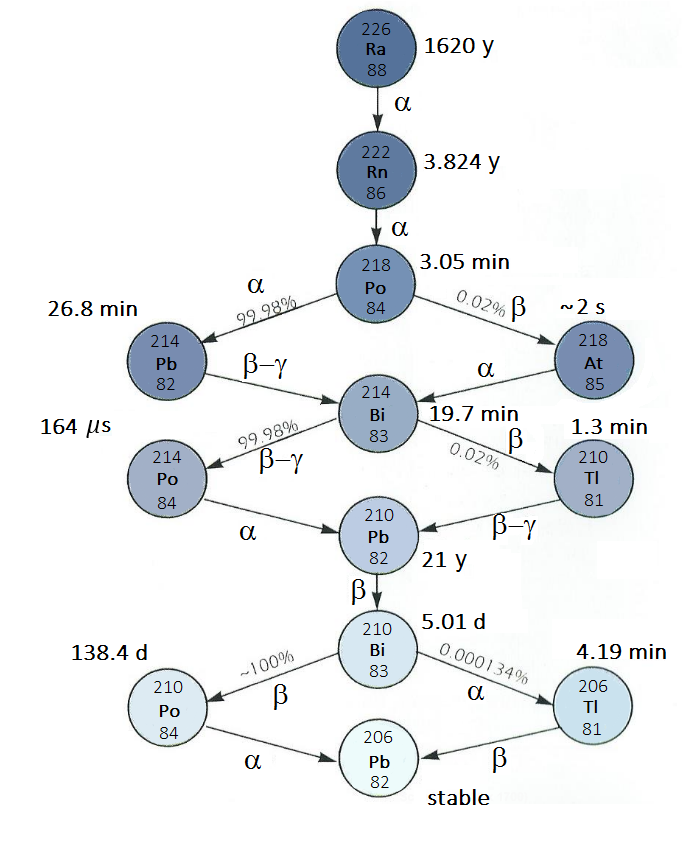
\includegraphics[scale=0.35]{figures/CadenaRn222.png}
\end{figure}


\end{frame}



\begin{frame}{Natural radioactivity}

\begin{itemize}
\item Since the Earth Earth’s birth 
\item Every second values are lower and lower : Exponential decay In our bodies 
\item $^{40}$K In the rocks, air, water, food, clothes, EVERYWHERE 
\item More than 50 \% of dose is NATURAL RADIATION
\end{itemize}

\begin{figure}
\centering
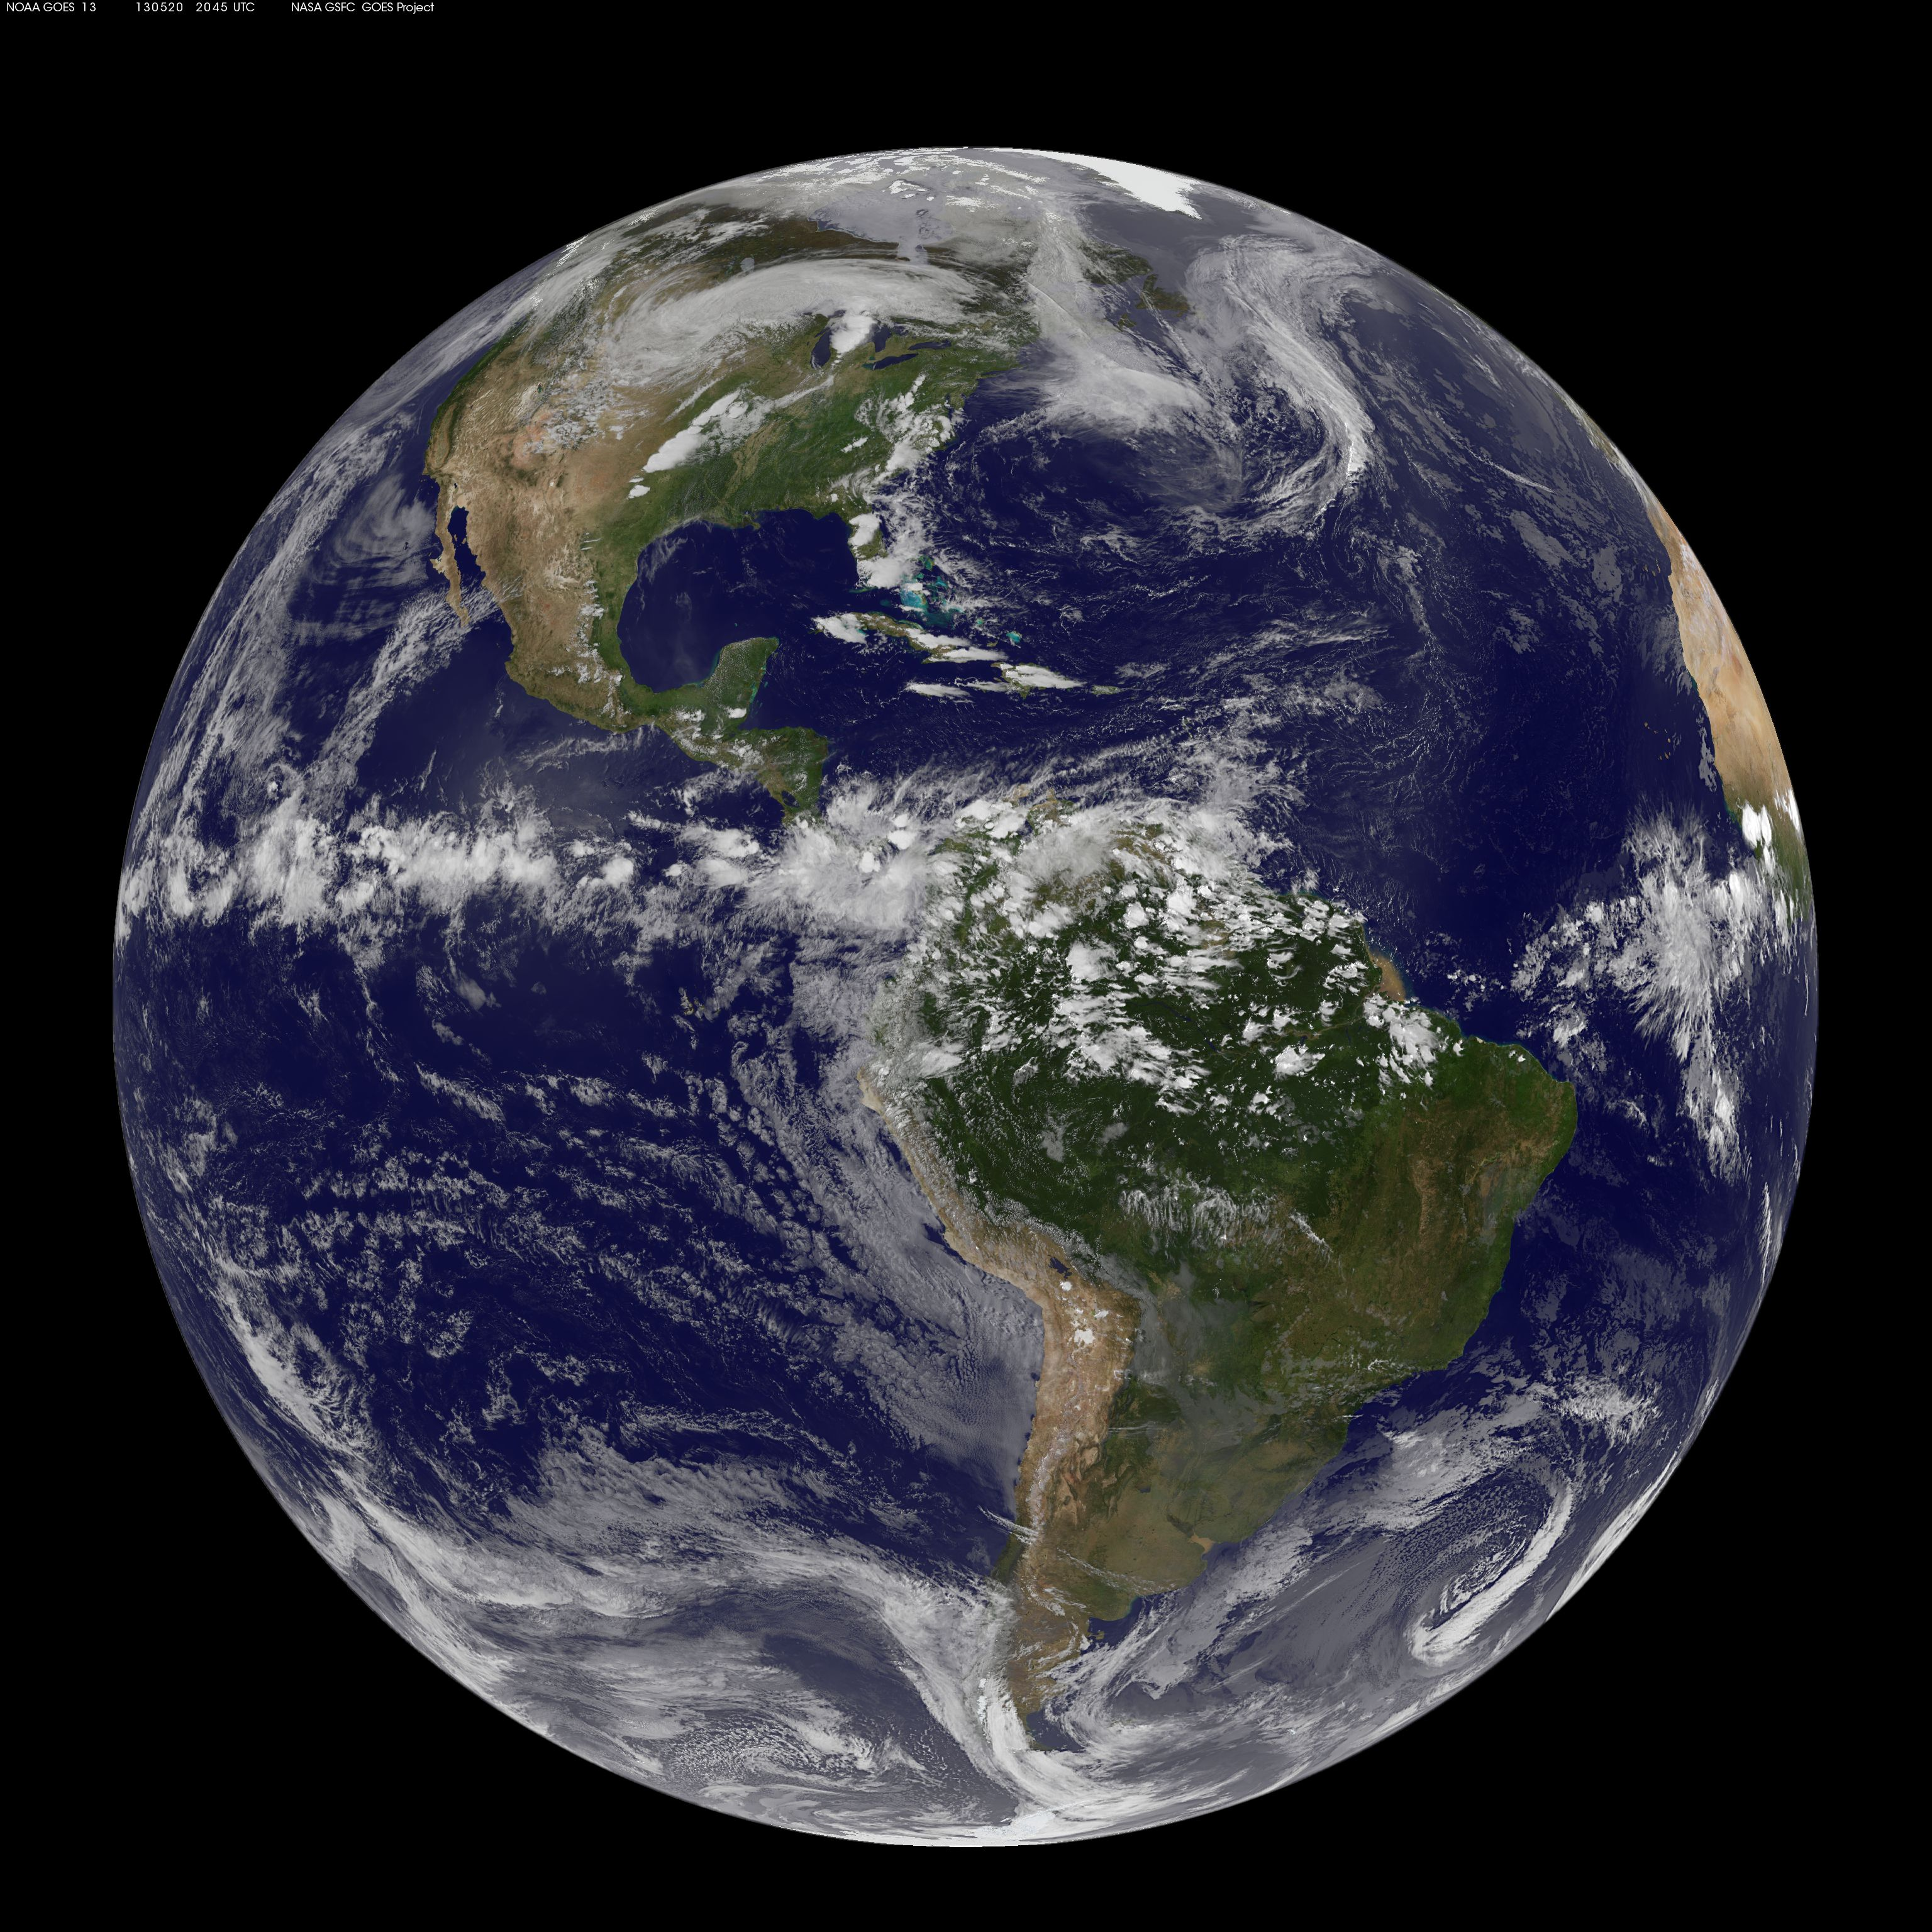
\includegraphics[scale=0.04]{figures/8770102292_eb5eca13b8_o}
\caption*{\href{https://www.flickr.com/photos/gsfc/}{\emph{Credit: 
NASA Goddard Space Flight Center
}}}
\end{figure}

\end{frame}

\begin{frame}{Natural radioactivity}

\centering
\alert{COSMIC RADIATION}

\begin{figure}
\centering
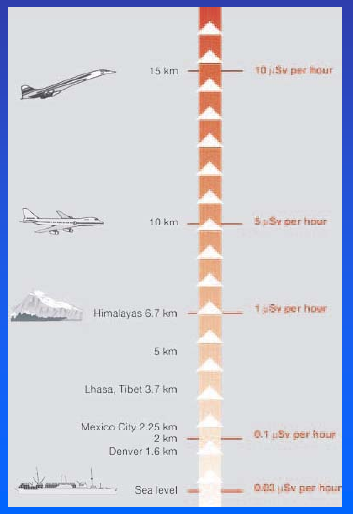
\includegraphics[scale=0.5]{figures/20160220_rsw_cosmicrad.png}
\caption*{\emph{Credit: Radiation, people and the environment (IAEA, February 2004)}}
\end{figure}

\end{frame}

\begin{frame}{Artificial radioactivity}

\begin{itemize}
\item Radioactive isotopes can be created 
\item Fission and fusion = Energy AND/OR destruction 
\item X-ray detectors 
\item Medical applications 
\item Industrial applications
\end{itemize}

\begin{table}
\begin{tabular}{cc}
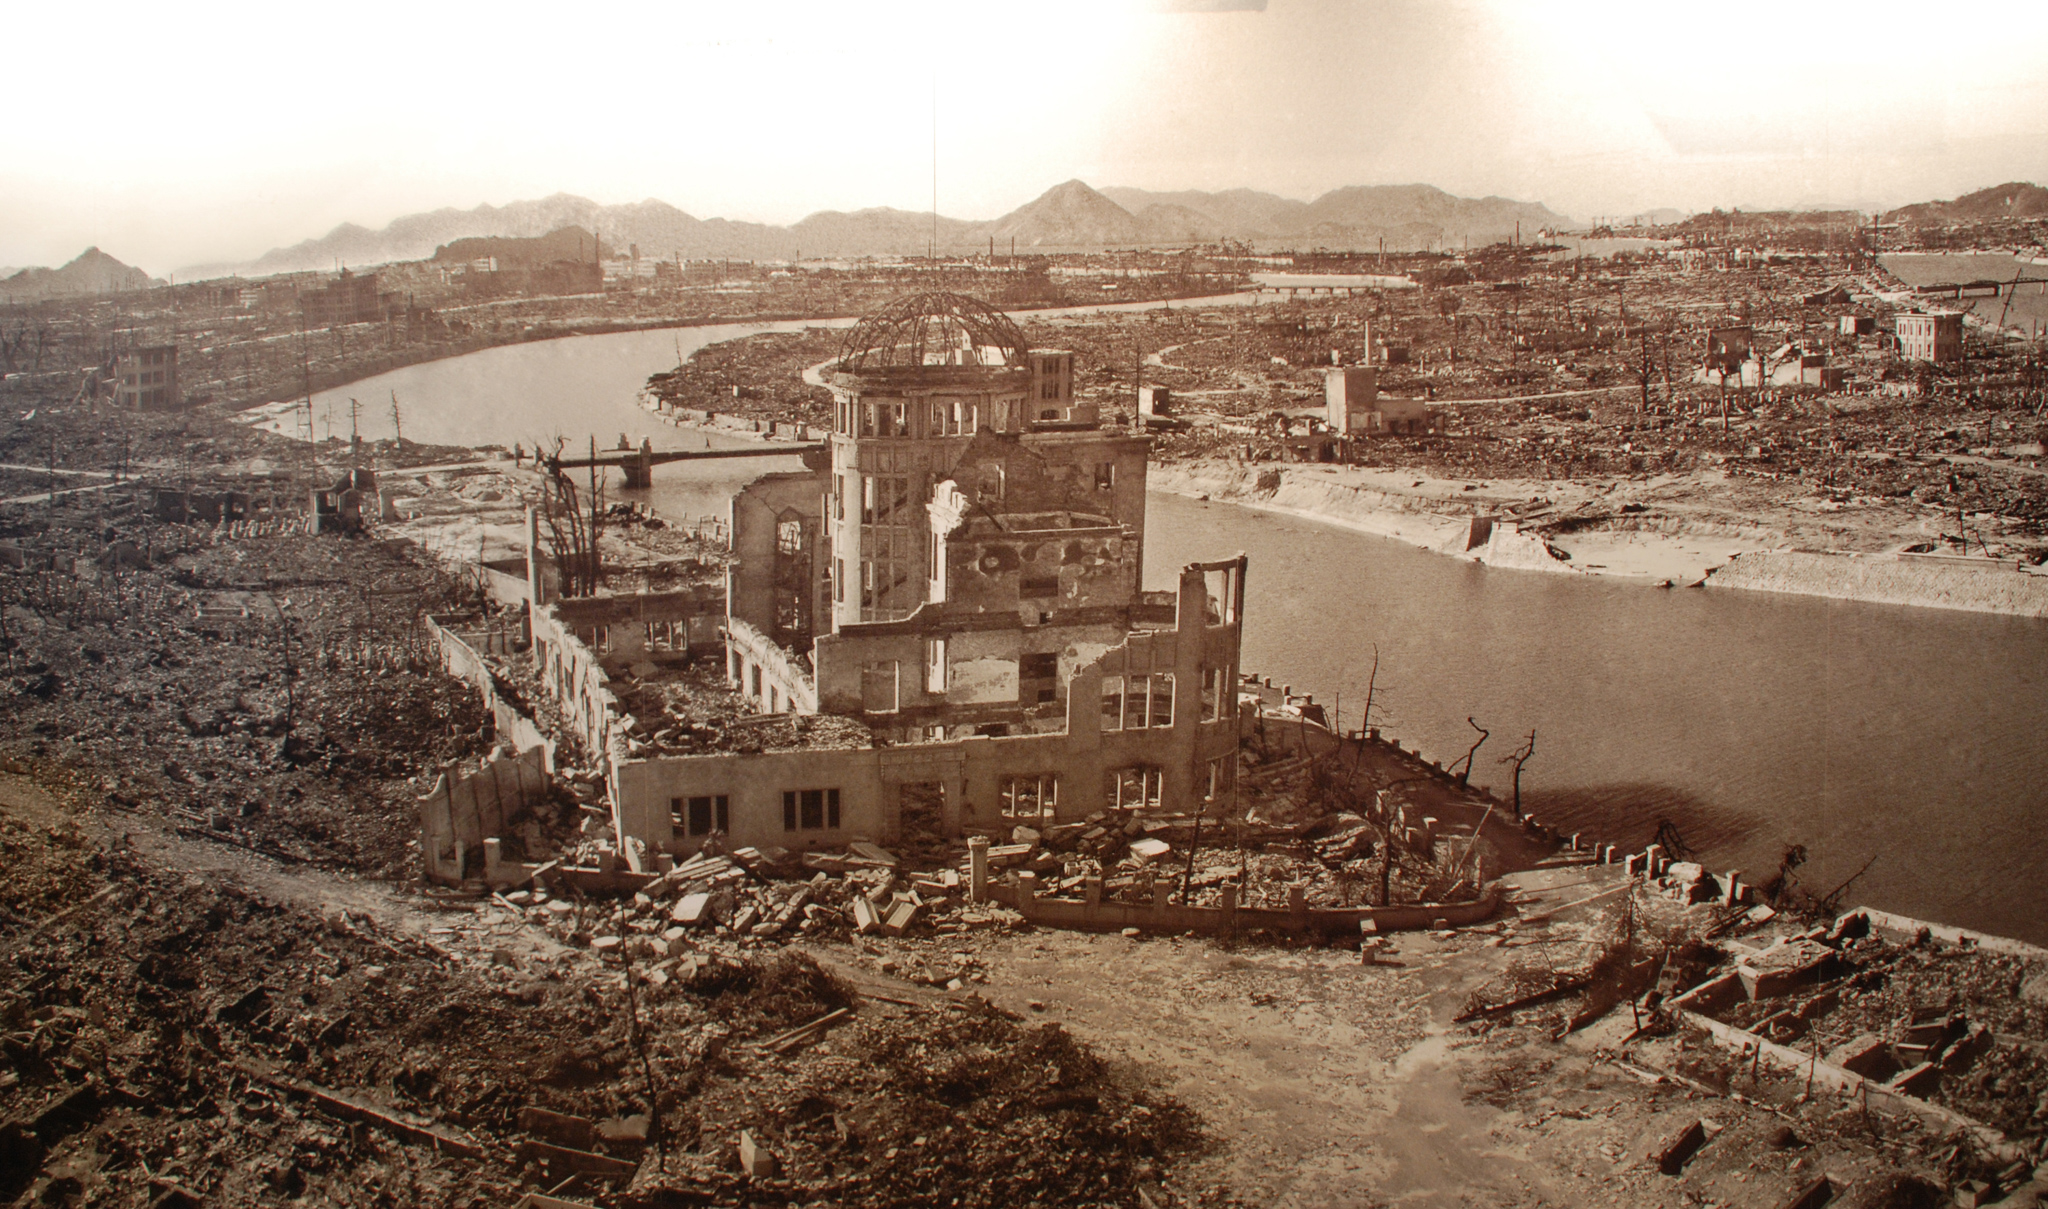
\includegraphics[scale=0.25]{figures/5105065678_df5d2fd6a2_o} & 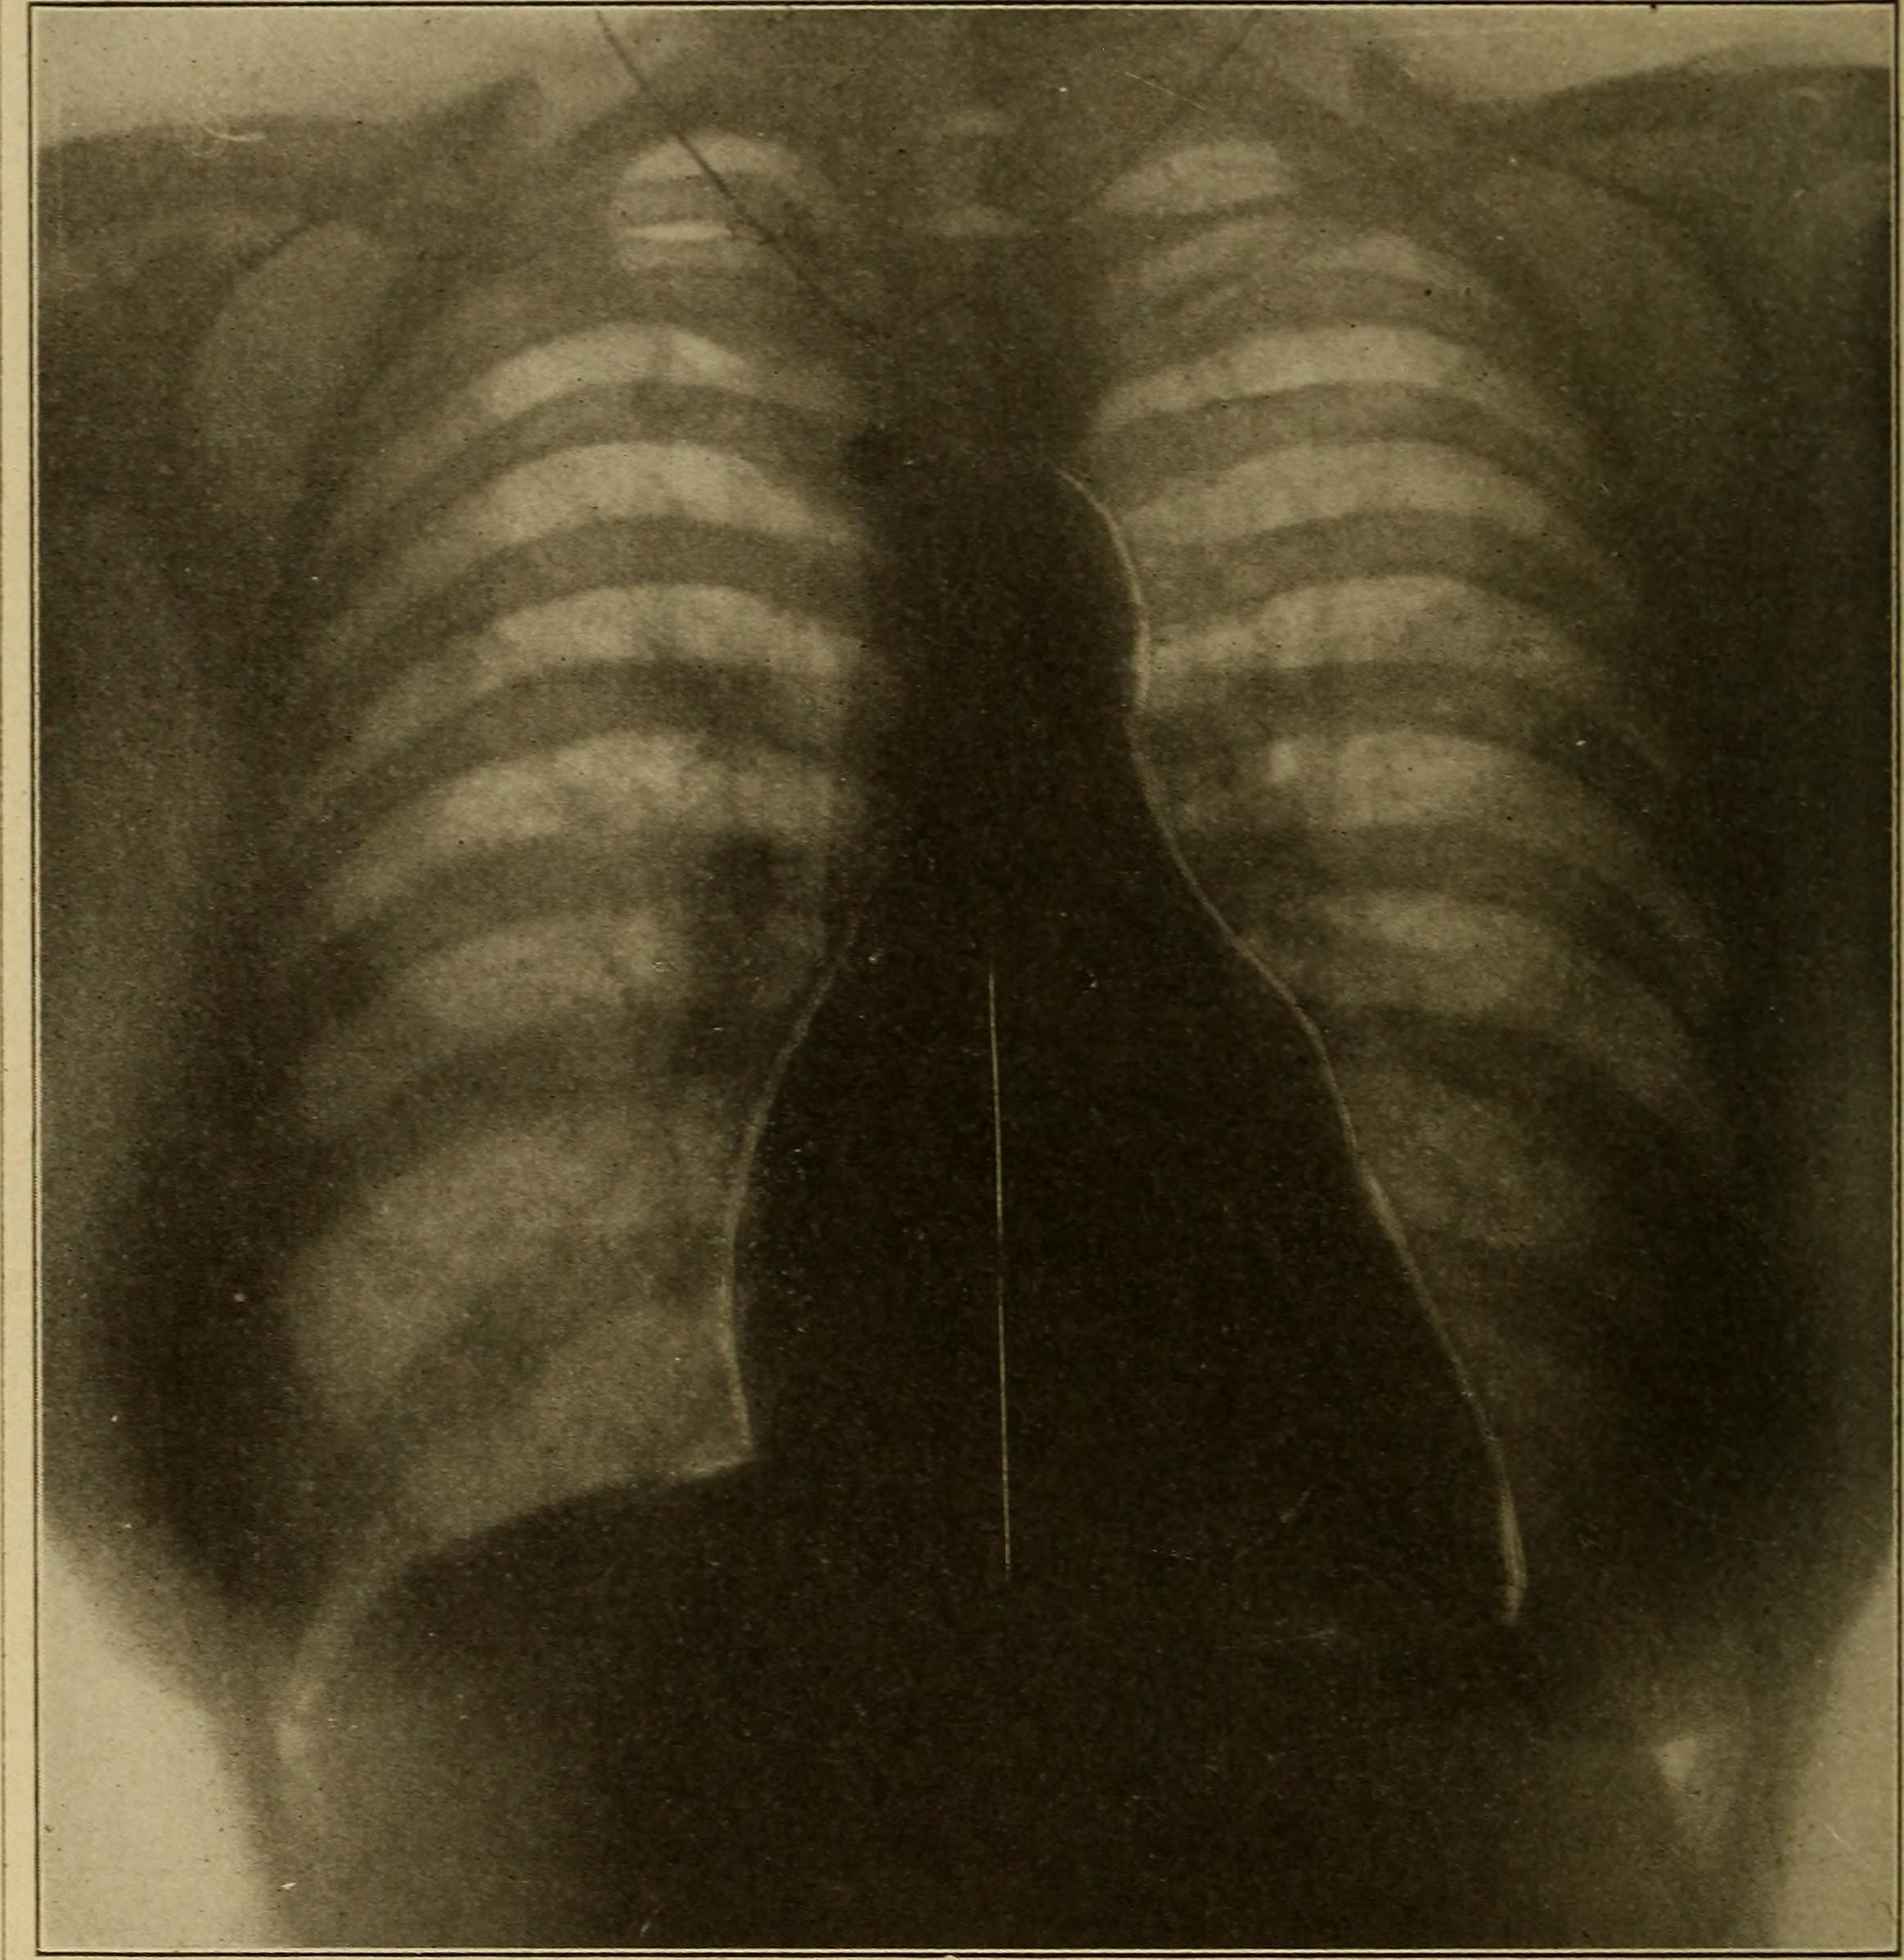
\includegraphics[scale=0.025]{figures/14781624461_49afb948a1_o} \\
\href{https://www.flickr.com/photos/xiquinho/}{\emph{Credit: 
Xiquinho Silva}} & 
\end{tabular}
\end{table}

\end{frame}

\begin{frame}{Learnings so far}

\begin{alertblock}{Let's remember}

\begin{itemize}

\pause \item Radiactivity: natural and artificial

\pause \item 3 decay modes: alpha, beta and gamma

\pause \item Units: activity (Bq, Ci); WLM

\pause \item  4 Natural decay series


\end{itemize}

\end{alertblock}

\end{frame}